\section{Physical Modelling}\label{sec:phy}
Physical Data Modeling (PDM) is the final step in data modeling. A PDM is primarily concerned with the implementation of a database-specific data model. As a result, it depicts how the model will be created in the database. For a non-technical individual, this data model is difficult to comprehend. This data model is required to create a query for CRUD activities.
We created a Physical Data Model based on Logical Data Modeling (LDM) and Normalization. We utilized the MYSQL database server and applied the FDM reconsideration to it in this case. The name convention for entities and attributes was "Snake Case." For example, we used "student id" for the attribute name "Student ID." The Physical Data Model we used in our MYSQL database server is shown below.\\

\begin{figure}[H]
    \centering
    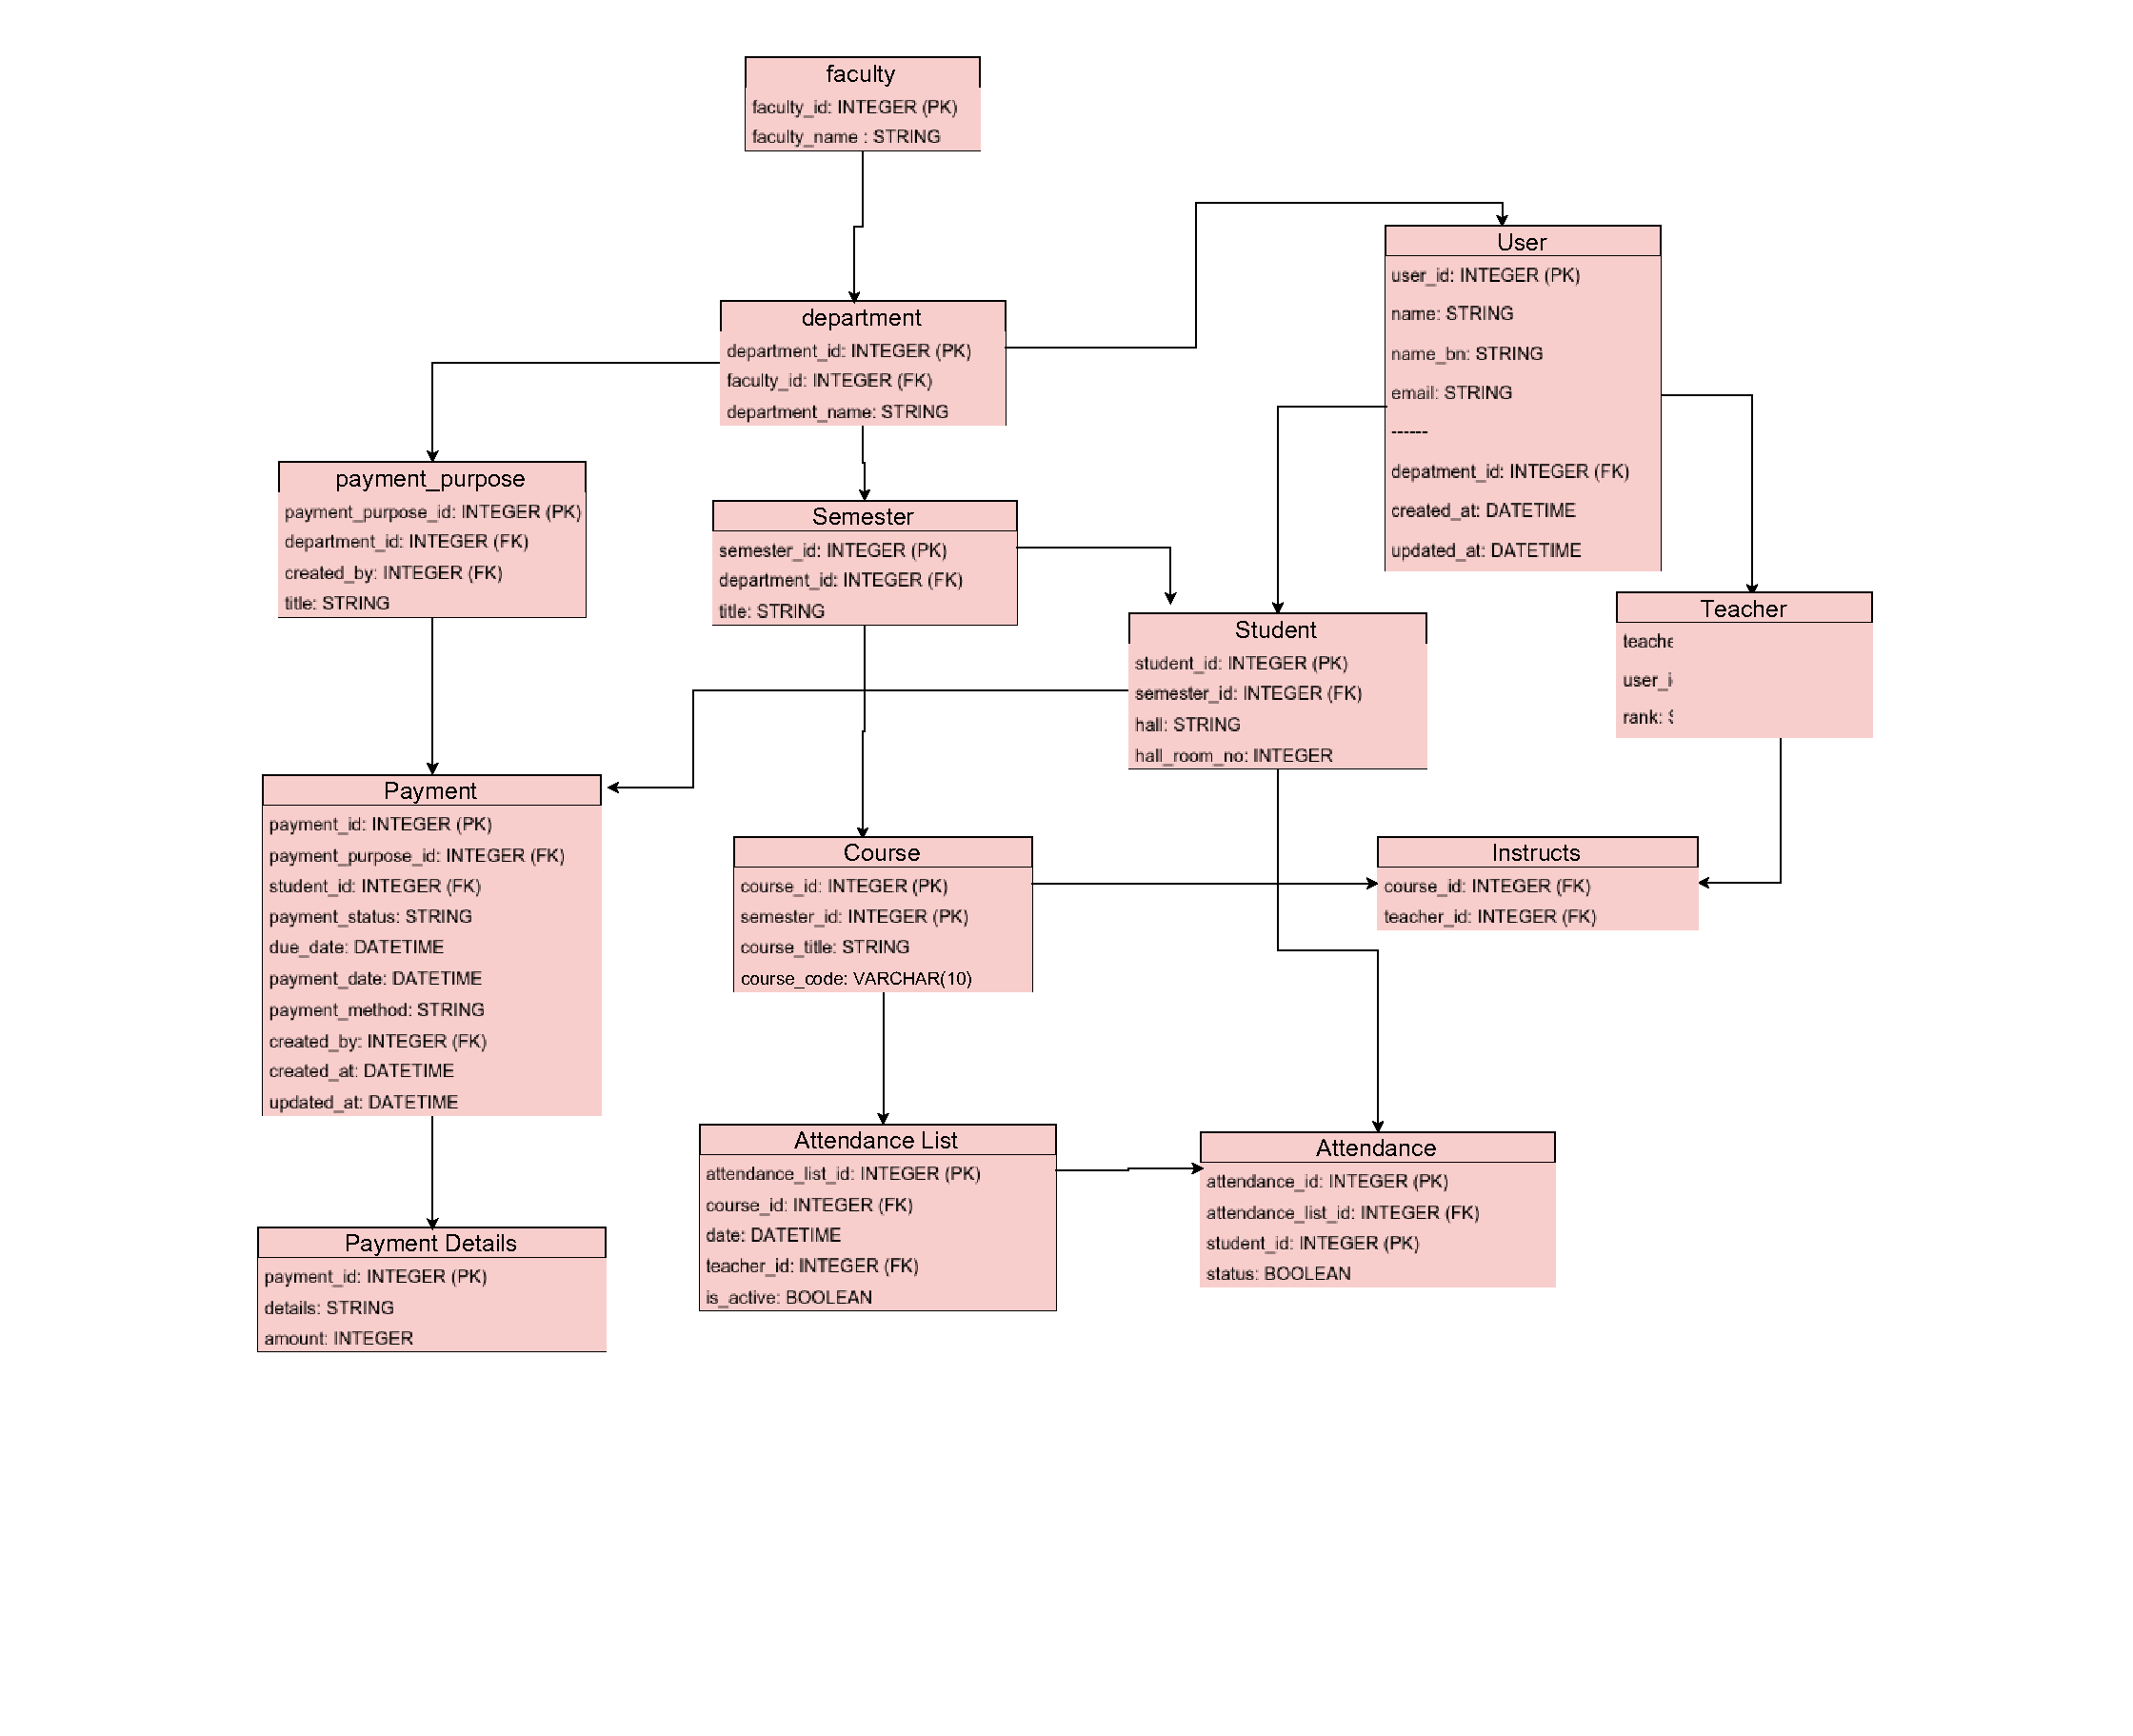
\includegraphics[width=1\textwidth]{images/physical}
    \caption{Physical Data Model of CU-OPAS}
    \label{fig:physical}
\end{figure}

Write a short description of Relation model. 
Write a how you convert your E-R model in Relational model
\clearpage